\documentclass[1p]{elsarticle_modified}
%\bibliographystyle{elsarticle-num}

%\usepackage[colorlinks]{hyperref}
%\usepackage{abbrmath_seonhwa} %\Abb, \Ascr, \Acal ,\Abf, \Afrak
\usepackage{amsfonts}
\usepackage{amssymb}
\usepackage{amsmath}
\usepackage{amsthm}
\usepackage{scalefnt}
\usepackage{amsbsy}
\usepackage{kotex}
\usepackage{caption}
\usepackage{subfig}
\usepackage{color}
\usepackage{graphicx}
\usepackage{xcolor} %% white, black, red, green, blue, cyan, magenta, yellow
\usepackage{float}
\usepackage{setspace}
\usepackage{hyperref}

\usepackage{tikz}
\usetikzlibrary{arrows}

\usepackage{multirow}
\usepackage{array} % fixed length table
\usepackage{hhline}

%%%%%%%%%%%%%%%%%%%%%
\makeatletter
\renewcommand*\env@matrix[1][\arraystretch]{%
	\edef\arraystretch{#1}%
	\hskip -\arraycolsep
	\let\@ifnextchar\new@ifnextchar
	\array{*\c@MaxMatrixCols c}}
\makeatother %https://tex.stackexchange.com/questions/14071/how-can-i-increase-the-line-spacing-in-a-matrix
%%%%%%%%%%%%%%%

\usepackage[normalem]{ulem}

\newcommand{\msout}[1]{\ifmmode\text{\sout{\ensuremath{#1}}}\else\sout{#1}\fi}
%SOURCE: \msout is \stkout macro in https://tex.stackexchange.com/questions/20609/strikeout-in-math-mode

\newcommand{\cancel}[1]{
	\ifmmode
	{\color{red}\msout{#1}}
	\else
	{\color{red}\sout{#1}}
	\fi
}

\newcommand{\add}[1]{
	{\color{blue}\uwave{#1}}
}

\newcommand{\replace}[2]{
	\ifmmode
	{\color{red}\msout{#1}}{\color{blue}\uwave{#2}}
	\else
	{\color{red}\sout{#1}}{\color{blue}\uwave{#2}}
	\fi
}

\newcommand{\Sol}{\mathcal{S}} %segment
\newcommand{\D}{D} %diagram
\newcommand{\A}{\mathcal{A}} %arc


%%%%%%%%%%%%%%%%%%%%%%%%%%%%%5 test

\def\sl{\operatorname{\textup{SL}}(2,\Cbb)}
\def\psl{\operatorname{\textup{PSL}}(2,\Cbb)}
\def\quan{\mkern 1mu \triangleright \mkern 1mu}

\theoremstyle{definition}
\newtheorem{thm}{Theorem}[section]
\newtheorem{prop}[thm]{Proposition}
\newtheorem{lem}[thm]{Lemma}
\newtheorem{ques}[thm]{Question}
\newtheorem{cor}[thm]{Corollary}
\newtheorem{defn}[thm]{Definition}
\newtheorem{exam}[thm]{Example}
\newtheorem{rmk}[thm]{Remark}
\newtheorem{alg}[thm]{Algorithm}

\newcommand{\I}{\sqrt{-1}}
\begin{document}

%\begin{frontmatter}
%
%\title{Boundary parabolic representations of knots up to 8 crossings}
%
%%% Group authors per affiliation:
%\author{Yunhi Cho} 
%\address{Department of Mathematics, University of Seoul, Seoul, Korea}
%\ead{yhcho@uos.ac.kr}
%
%
%\author{Seonhwa Kim} %\fnref{s_kim}}
%\address{Center for Geometry and Physics, Institute for Basic Science, Pohang, 37673, Korea}
%\ead{ryeona17@ibs.re.kr}
%
%\author{Hyuk Kim}
%\address{Department of Mathematical Sciences, Seoul National University, Seoul 08826, Korea}
%\ead{hyukkim@snu.ac.kr}
%
%\author{Seokbeom Yoon}
%\address{Department of Mathematical Sciences, Seoul National University, Seoul, 08826,  Korea}
%\ead{sbyoon15@snu.ac.kr}
%
%\begin{abstract}
%We find all boundary parabolic representation of knots up to 8 crossings.
%
%\end{abstract}
%\begin{keyword}
%    \MSC[2010] 57M25 
%\end{keyword}
%
%\end{frontmatter}

%\linenumbers
%\tableofcontents
%
\newcommand\colored[1]{\textcolor{white}{\rule[-0.35ex]{0.8em}{1.4ex}}\kern-0.8em\color{red} #1}%
%\newcommand\colored[1]{\textcolor{white}{ #1}\kern-2.17ex	\textcolor{white}{ #1}\kern-1.81ex	\textcolor{white}{ #1}\kern-2.15ex\color{red}#1	}

{\Large $\underline{12a_{0091}~(K12a_{0091})}$}

\setlength{\tabcolsep}{10pt}
\renewcommand{\arraystretch}{1.6}
\vspace{1cm}\begin{tabular}{m{100pt}>{\centering\arraybackslash}m{274pt}}
\multirow{5}{120pt}{
	\centering
	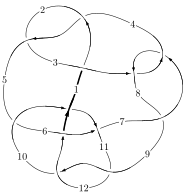
\includegraphics[width=112pt]{../../../GIT/diagram.site/Diagrams/png/892_12a_0091.png}\\
\ \ \ A knot diagram\footnotemark}&
\allowdisplaybreaks
\textbf{Linearized knot diagam} \\
\cline{2-2}
 &
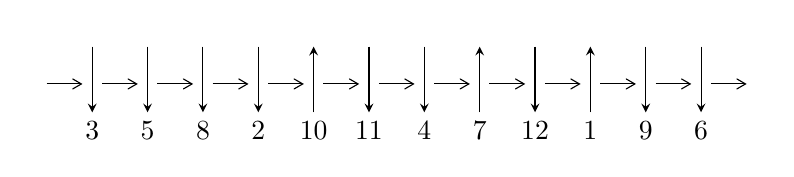
\begin{tikzpicture}[x=20pt, y=17pt]
	% nodes
	\node (C0) at (0, 0) {};
	\node (C1) at (1, 0) {};
	\node (C1U) at (1, +1) {};
	\node (C1D) at (1, -1) {3};

	\node (C2) at (2, 0) {};
	\node (C2U) at (2, +1) {};
	\node (C2D) at (2, -1) {5};

	\node (C3) at (3, 0) {};
	\node (C3U) at (3, +1) {};
	\node (C3D) at (3, -1) {8};

	\node (C4) at (4, 0) {};
	\node (C4U) at (4, +1) {};
	\node (C4D) at (4, -1) {2};

	\node (C5) at (5, 0) {};
	\node (C5U) at (5, +1) {};
	\node (C5D) at (5, -1) {10};

	\node (C6) at (6, 0) {};
	\node (C6U) at (6, +1) {};
	\node (C6D) at (6, -1) {11};

	\node (C7) at (7, 0) {};
	\node (C7U) at (7, +1) {};
	\node (C7D) at (7, -1) {4};

	\node (C8) at (8, 0) {};
	\node (C8U) at (8, +1) {};
	\node (C8D) at (8, -1) {7};

	\node (C9) at (9, 0) {};
	\node (C9U) at (9, +1) {};
	\node (C9D) at (9, -1) {12};

	\node (C10) at (10, 0) {};
	\node (C10U) at (10, +1) {};
	\node (C10D) at (10, -1) {1};

	\node (C11) at (11, 0) {};
	\node (C11U) at (11, +1) {};
	\node (C11D) at (11, -1) {9};

	\node (C12) at (12, 0) {};
	\node (C12U) at (12, +1) {};
	\node (C12D) at (12, -1) {6};
	\node (C13) at (13, 0) {};

	% arrows
	\draw[->,>={angle 60}]
	(C0) edge (C1) (C1) edge (C2) (C2) edge (C3) (C3) edge (C4) (C4) edge (C5) (C5) edge (C6) (C6) edge (C7) (C7) edge (C8) (C8) edge (C9) (C9) edge (C10) (C10) edge (C11) (C11) edge (C12) (C12) edge (C13) ;	\draw[->,>=stealth]
	(C1U) edge (C1D) (C2U) edge (C2D) (C3U) edge (C3D) (C4U) edge (C4D) (C5D) edge (C5U) (C6U) edge (C6D) (C7U) edge (C7D) (C8D) edge (C8U) (C9U) edge (C9D) (C10D) edge (C10U) (C11U) edge (C11D) (C12U) edge (C12D) ;
	\end{tikzpicture} \\
\hhline{~~} \\& 
\textbf{Solving Sequence} \\ \cline{2-2} 
 &
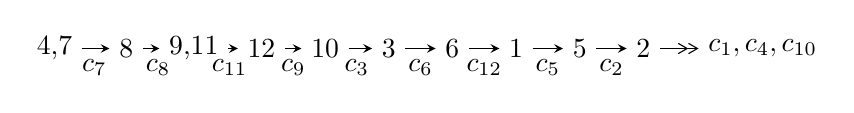
\begin{tikzpicture}[x=23pt, y=7pt]
	% node
	\node (A0) at (-1/8, 0) {4,7};
	\node (A1) at (1, 0) {8};
	\node (A2) at (33/16, 0) {9,11};
	\node (A3) at (25/8, 0) {12};
	\node (A4) at (33/8, 0) {10};
	\node (A5) at (41/8, 0) {3};
	\node (A6) at (49/8, 0) {6};
	\node (A7) at (57/8, 0) {1};
	\node (A8) at (65/8, 0) {5};
	\node (A9) at (73/8, 0) {2};
	\node (C1) at (1/2, -1) {$c_{7}$};
	\node (C2) at (3/2, -1) {$c_{8}$};
	\node (C3) at (21/8, -1) {$c_{11}$};
	\node (C4) at (29/8, -1) {$c_{9}$};
	\node (C5) at (37/8, -1) {$c_{3}$};
	\node (C6) at (45/8, -1) {$c_{6}$};
	\node (C7) at (53/8, -1) {$c_{12}$};
	\node (C8) at (61/8, -1) {$c_{5}$};
	\node (C9) at (69/8, -1) {$c_{2}$};
	\node (A10) at (11, 0) {$c_{1},c_{4},c_{10}$};

	% edge
	\draw[->,>=stealth]	
	(A0) edge (A1) (A1) edge (A2) (A2) edge (A3) (A3) edge (A4) (A4) edge (A5) (A5) edge (A6) (A6) edge (A7) (A7) edge (A8) (A8) edge (A9) ;
	\draw[->>,>={angle 60}]	
	(A9) edge (A10);
\end{tikzpicture} \\ 

\end{tabular} \\

\footnotetext{
The image of knot diagram is generated by the software ``\textbf{Draw programme}" developed by Andrew Bartholomew(\url{http://www.layer8.co.uk/maths/draw/index.htm\#Running-draw}), where we modified some parts for our purpose(\url{https://github.com/CATsTAILs/LinksPainter}).
}\phantom \\ \newline 
\centering \textbf{Ideals for irreducible components\footnotemark of $X_{\text{par}}$} 
 
\begin{align*}
I^u_{1}&=\langle 
1.40905\times10^{271} u^{117}-3.19731\times10^{271} u^{116}+\cdots+1.57559\times10^{272} b-8.05247\times10^{272},\\
\phantom{I^u_{1}}&\phantom{= \langle  }1.79454\times10^{272} u^{117}-3.91278\times10^{272} u^{116}+\cdots+3.15118\times10^{272} a-5.43779\times10^{273},\\
\phantom{I^u_{1}}&\phantom{= \langle  }u^{118}-2 u^{117}+\cdots-160 u+32\rangle \\
I^u_{2}&=\langle 
-2 u^2+b- u-3,\;-5 u^2+a-2 u-9,\;u^3+u^2+2 u+1\rangle \\
\\
I^v_{1}&=\langle 
a,\;v^4+12 v^3+24 v^2+29 b+21 v+45,\;v^5+3 v^4+3 v^3+8 v^2+v+1\rangle \\
\end{align*}
\raggedright * 3 irreducible components of $\dim_{\mathbb{C}}=0$, with total 126 representations.\\
\footnotetext{All coefficients of polynomials are rational numbers. But the coefficients are sometimes approximated in decimal forms when there is not enough margin.}
\newpage
\renewcommand{\arraystretch}{1}
\centering \section*{I. $I^u_{1}= \langle 1.41\times10^{271} u^{117}-3.20\times10^{271} u^{116}+\cdots+1.58\times10^{272} b-8.05\times10^{272},\;1.79\times10^{272} u^{117}-3.91\times10^{272} u^{116}+\cdots+3.15\times10^{272} a-5.44\times10^{273},\;u^{118}-2 u^{117}+\cdots-160 u+32 \rangle$}
\flushleft \textbf{(i) Arc colorings}\\
\begin{tabular}{m{7pt} m{180pt} m{7pt} m{180pt} }
\flushright $a_{4}=$&$\begin{pmatrix}0\\u\end{pmatrix}$ \\
\flushright $a_{7}=$&$\begin{pmatrix}1\\0\end{pmatrix}$ \\
\flushright $a_{8}=$&$\begin{pmatrix}1\\u^2\end{pmatrix}$ \\
\flushright $a_{9}=$&$\begin{pmatrix}u^2+1\\u^2\end{pmatrix}$ \\
\flushright $a_{11}=$&$\begin{pmatrix}-0.569481 u^{117}+1.24169 u^{116}+\cdots-133.388 u+17.2564\\-0.0894301 u^{117}+0.202928 u^{116}+\cdots-39.7435 u+5.11076\end{pmatrix}$ \\
\flushright $a_{12}=$&$\begin{pmatrix}-0.373615 u^{117}+0.817065 u^{116}+\cdots-78.1427 u+10.4088\\-0.160556 u^{117}+0.336670 u^{116}+\cdots-52.1880 u+5.89092\end{pmatrix}$ \\
\flushright $a_{10}=$&$\begin{pmatrix}-0.255516 u^{117}+0.458821 u^{116}+\cdots-5.26560 u-0.632464\\0.187447 u^{117}-0.419386 u^{116}+\cdots+67.1265 u-6.07320\end{pmatrix}$ \\
\flushright $a_{3}=$&$\begin{pmatrix}u\\u^3+u\end{pmatrix}$ \\
\flushright $a_{6}=$&$\begin{pmatrix}-0.321859 u^{117}+0.588545 u^{116}+\cdots-26.5015 u-3.74902\\-0.120061 u^{117}+0.303595 u^{116}+\cdots-65.4915 u+7.49794\end{pmatrix}$ \\
\flushright $a_{1}=$&$\begin{pmatrix}-0.381325 u^{117}+0.734164 u^{116}+\cdots-16.2430 u-2.30564\\-0.0732515 u^{117}+0.0465062 u^{116}+\cdots+69.4204 u-15.1813\end{pmatrix}$ \\
\flushright $a_{5}=$&$\begin{pmatrix}-0.161618 u^{117}+0.417138 u^{116}+\cdots-78.0186 u+13.7872\\0.219707 u^{117}-0.317027 u^{116}+\cdots-61.7756 u+16.0928\end{pmatrix}$ \\
\flushright $a_{2}=$&$\begin{pmatrix}-0.305156 u^{117}+0.565775 u^{116}+\cdots+3.95305 u-5.31050\\-0.0281133 u^{117}-0.0595301 u^{116}+\cdots+84.6108 u-17.6725\end{pmatrix}$\\&\end{tabular}
\flushleft \textbf{(ii) Obstruction class $= -1$}\\~\\
\flushleft \textbf{(iii) Cusp Shapes $= 0.287760 u^{117}-0.227055 u^{116}+\cdots-36.3944 u+24.9413$}\\~\\
\newpage\renewcommand{\arraystretch}{1}
\flushleft \textbf{(iv) u-Polynomials at the component}\newline \\
\begin{tabular}{m{50pt}|m{274pt}}
Crossings & \hspace{64pt}u-Polynomials at each crossing \\
\hline $$\begin{aligned}c_{1}\end{aligned}$$&$\begin{aligned}
&u^{118}+65 u^{117}+\cdots+172 u+1
\end{aligned}$\\
\hline $$\begin{aligned}c_{2},c_{4}\end{aligned}$$&$\begin{aligned}
&u^{118}-7 u^{117}+\cdots-2 u+1
\end{aligned}$\\
\hline $$\begin{aligned}c_{3},c_{7}\end{aligned}$$&$\begin{aligned}
&u^{118}+2 u^{117}+\cdots+160 u+32
\end{aligned}$\\
\hline $$\begin{aligned}c_{5}\end{aligned}$$&$\begin{aligned}
&u^{118}+67 u^{116}+\cdots+196401 u+29189
\end{aligned}$\\
\hline $$\begin{aligned}c_{6}\end{aligned}$$&$\begin{aligned}
&u^{118}+4 u^{117}+\cdots+8634757 u+591517
\end{aligned}$\\
\hline $$\begin{aligned}c_{8}\end{aligned}$$&$\begin{aligned}
&u^{118}-36 u^{117}+\cdots-20992 u+1024
\end{aligned}$\\
\hline $$\begin{aligned}c_{9},c_{11}\end{aligned}$$&$\begin{aligned}
&u^{118}-5 u^{117}+\cdots+143 u-1
\end{aligned}$\\
\hline $$\begin{aligned}c_{10}\end{aligned}$$&$\begin{aligned}
&u^{118}+20 u^{117}+\cdots+156 u+8
\end{aligned}$\\
\hline $$\begin{aligned}c_{12}\end{aligned}$$&$\begin{aligned}
&u^{118}-9 u^{117}+\cdots+2 u-1
\end{aligned}$\\
\hline
\end{tabular}\\~\\
\newpage\renewcommand{\arraystretch}{1}
\flushleft \textbf{(v) Riley Polynomials at the component}\newline \\
\begin{tabular}{m{50pt}|m{274pt}}
Crossings & \hspace{64pt}Riley Polynomials at each crossing \\
\hline $$\begin{aligned}c_{1}\end{aligned}$$&$\begin{aligned}
&y^{118}-17 y^{117}+\cdots-21024 y+1
\end{aligned}$\\
\hline $$\begin{aligned}c_{2},c_{4}\end{aligned}$$&$\begin{aligned}
&y^{118}-65 y^{117}+\cdots-172 y+1
\end{aligned}$\\
\hline $$\begin{aligned}c_{3},c_{7}\end{aligned}$$&$\begin{aligned}
&y^{118}+36 y^{117}+\cdots+20992 y+1024
\end{aligned}$\\
\hline $$\begin{aligned}c_{5}\end{aligned}$$&$\begin{aligned}
&y^{118}+134 y^{117}+\cdots+56845137931 y+851997721
\end{aligned}$\\
\hline $$\begin{aligned}c_{6}\end{aligned}$$&$\begin{aligned}
&y^{118}+46 y^{117}+\cdots-9372454336793 y+349892361289
\end{aligned}$\\
\hline $$\begin{aligned}c_{8}\end{aligned}$$&$\begin{aligned}
&y^{118}+84 y^{117}+\cdots-237633536 y+1048576
\end{aligned}$\\
\hline $$\begin{aligned}c_{9},c_{11}\end{aligned}$$&$\begin{aligned}
&y^{118}-91 y^{117}+\cdots-21455 y+1
\end{aligned}$\\
\hline $$\begin{aligned}c_{10}\end{aligned}$$&$\begin{aligned}
&y^{118}+24 y^{117}+\cdots-6288 y+64
\end{aligned}$\\
\hline $$\begin{aligned}c_{12}\end{aligned}$$&$\begin{aligned}
&y^{118}-25 y^{117}+\cdots-26 y+1
\end{aligned}$\\
\hline
\end{tabular}\\~\\
\newpage\flushleft \textbf{(vi) Complex Volumes and Cusp Shapes}
$$\begin{array}{c|c|c}  
\text{Solutions to }I^u_{1}& \I (\text{vol} + \sqrt{-1}CS) & \text{Cusp shape}\\
 \hline 
\begin{aligned}
u &= -0.728017 + 0.694463 I \\
a &= \phantom{-}1.47342 + 0.86530 I \\
b &= \phantom{-}0.767924 + 0.400602 I\end{aligned}
 & -1.43969 - 2.21556 I & \phantom{-0.000000 } 0 \\ \hline\begin{aligned}
u &= -0.728017 - 0.694463 I \\
a &= \phantom{-}1.47342 - 0.86530 I \\
b &= \phantom{-}0.767924 - 0.400602 I\end{aligned}
 & -1.43969 + 2.21556 I & \phantom{-0.000000 } 0 \\ \hline\begin{aligned}
u &= \phantom{-}0.619537 + 0.765048 I \\
a &= \phantom{-}1.78016 + 0.17358 I \\
b &= \phantom{-}0.818692 + 0.835076 I\end{aligned}
 & -1.23232 - 1.59626 I & \phantom{-0.000000 } 0 \\ \hline\begin{aligned}
u &= \phantom{-}0.619537 - 0.765048 I \\
a &= \phantom{-}1.78016 - 0.17358 I \\
b &= \phantom{-}0.818692 - 0.835076 I\end{aligned}
 & -1.23232 + 1.59626 I & \phantom{-0.000000 } 0 \\ \hline\begin{aligned}
u &= -0.298455 + 0.934841 I \\
a &= \phantom{-}0.29656 - 1.43402 I \\
b &= -0.263877 + 0.281634 I\end{aligned}
 & -1.47083 + 5.17351 I & \phantom{-0.000000 } 0 \\ \hline\begin{aligned}
u &= -0.298455 - 0.934841 I \\
a &= \phantom{-}0.29656 + 1.43402 I \\
b &= -0.263877 - 0.281634 I\end{aligned}
 & -1.47083 - 5.17351 I & \phantom{-0.000000 } 0 \\ \hline\begin{aligned}
u &= \phantom{-}0.198124 + 0.953787 I \\
a &= -0.264398 + 0.390388 I \\
b &= \phantom{-}0.12045 - 2.76563 I\end{aligned}
 & \phantom{-}0.04031 - 2.55048 I & \phantom{-0.000000 } 0 \\ \hline\begin{aligned}
u &= \phantom{-}0.198124 - 0.953787 I \\
a &= -0.264398 - 0.390388 I \\
b &= \phantom{-}0.12045 + 2.76563 I\end{aligned}
 & \phantom{-}0.04031 + 2.55048 I & \phantom{-0.000000 } 0 \\ \hline\begin{aligned}
u &= -0.068591 + 0.971611 I \\
a &= -1.225790 + 0.651510 I \\
b &= \phantom{-}0.974512 - 0.440905 I\end{aligned}
 & -5.08436 + 4.73741 I & \phantom{-0.000000 } 0 \\ \hline\begin{aligned}
u &= -0.068591 - 0.971611 I \\
a &= -1.225790 - 0.651510 I \\
b &= \phantom{-}0.974512 + 0.440905 I\end{aligned}
 & -5.08436 - 4.73741 I & \phantom{-0.000000 } 0\\
 \hline 
 \end{array}$$\newpage$$\begin{array}{c|c|c}  
\text{Solutions to }I^u_{1}& \I (\text{vol} + \sqrt{-1}CS) & \text{Cusp shape}\\
 \hline 
\begin{aligned}
u &= -1.031110 + 0.197972 I \\
a &= -0.688682 - 0.721892 I \\
b &= -0.985148 - 0.601427 I\end{aligned}
 & -3.61891 - 7.05319 I & \phantom{-0.000000 } 0 \\ \hline\begin{aligned}
u &= -1.031110 - 0.197972 I \\
a &= -0.688682 + 0.721892 I \\
b &= -0.985148 + 0.601427 I\end{aligned}
 & -3.61891 + 7.05319 I & \phantom{-0.000000 } 0 \\ \hline\begin{aligned}
u &= \phantom{-}1.050710 + 0.063861 I \\
a &= -0.544435 - 0.438588 I \\
b &= -0.843272 - 0.325269 I\end{aligned}
 & -3.31472 - 2.51883 I & \phantom{-0.000000 } 0 \\ \hline\begin{aligned}
u &= \phantom{-}1.050710 - 0.063861 I \\
a &= -0.544435 + 0.438588 I \\
b &= -0.843272 + 0.325269 I\end{aligned}
 & -3.31472 + 2.51883 I & \phantom{-0.000000 } 0 \\ \hline\begin{aligned}
u &= -0.272135 + 1.025000 I \\
a &= \phantom{-}0.308053 + 0.319914 I \\
b &= -0.256239 - 0.968837 I\end{aligned}
 & \phantom{-}3.78308 + 0.01802 I & \phantom{-0.000000 } 0 \\ \hline\begin{aligned}
u &= -0.272135 - 1.025000 I \\
a &= \phantom{-}0.308053 - 0.319914 I \\
b &= -0.256239 + 0.968837 I\end{aligned}
 & \phantom{-}3.78308 - 0.01802 I & \phantom{-0.000000 } 0 \\ \hline\begin{aligned}
u &= -0.735517 + 0.778817 I \\
a &= -0.61695 - 1.66149 I \\
b &= -0.955699 - 0.607070 I\end{aligned}
 & -4.73869 - 0.40842 I & \phantom{-0.000000 } 0 \\ \hline\begin{aligned}
u &= -0.735517 - 0.778817 I \\
a &= -0.61695 + 1.66149 I \\
b &= -0.955699 + 0.607070 I\end{aligned}
 & -4.73869 + 0.40842 I & \phantom{-0.000000 } 0 \\ \hline\begin{aligned}
u &= \phantom{-}0.107153 + 1.069730 I \\
a &= -0.597452 + 0.680996 I \\
b &= -0.573835 - 0.928627 I\end{aligned}
 & \phantom{-}4.36870 - 2.02817 I & \phantom{-0.000000 } 0 \\ \hline\begin{aligned}
u &= \phantom{-}0.107153 - 1.069730 I \\
a &= -0.597452 - 0.680996 I \\
b &= -0.573835 + 0.928627 I\end{aligned}
 & \phantom{-}4.36870 + 2.02817 I & \phantom{-0.000000 } 0\\
 \hline 
 \end{array}$$\newpage$$\begin{array}{c|c|c}  
\text{Solutions to }I^u_{1}& \I (\text{vol} + \sqrt{-1}CS) & \text{Cusp shape}\\
 \hline 
\begin{aligned}
u &= -0.781234 + 0.740647 I \\
a &= -0.934177 - 0.255699 I \\
b &= -1.238870 - 0.360891 I\end{aligned}
 & -10.10770 + 4.91047 I & \phantom{-0.000000 } 0 \\ \hline\begin{aligned}
u &= -0.781234 - 0.740647 I \\
a &= -0.934177 + 0.255699 I \\
b &= -1.238870 + 0.360891 I\end{aligned}
 & -10.10770 - 4.91047 I & \phantom{-0.000000 } 0 \\ \hline\begin{aligned}
u &= \phantom{-}0.073380 + 0.920134 I \\
a &= \phantom{-}1.340470 - 0.353995 I \\
b &= \phantom{-}0.22772 + 2.02067 I\end{aligned}
 & \phantom{-}0.35506 - 1.51453 I & \phantom{-0.000000 } 0 \\ \hline\begin{aligned}
u &= \phantom{-}0.073380 - 0.920134 I \\
a &= \phantom{-}1.340470 + 0.353995 I \\
b &= \phantom{-}0.22772 - 2.02067 I\end{aligned}
 & \phantom{-}0.35506 + 1.51453 I & \phantom{-0.000000 } 0 \\ \hline\begin{aligned}
u &= \phantom{-}0.149078 + 1.079460 I \\
a &= -0.299400 + 0.181175 I \\
b &= -0.577685 - 0.021582 I\end{aligned}
 & \phantom{-}2.39623 - 2.35738 I & \phantom{-0.000000 } 0 \\ \hline\begin{aligned}
u &= \phantom{-}0.149078 - 1.079460 I \\
a &= -0.299400 - 0.181175 I \\
b &= -0.577685 + 0.021582 I\end{aligned}
 & \phantom{-}2.39623 + 2.35738 I & \phantom{-0.000000 } 0 \\ \hline\begin{aligned}
u &= \phantom{-}0.774685 + 0.781985 I \\
a &= -1.34750 + 0.88167 I \\
b &= -1.62710 + 0.76393 I\end{aligned}
 & -10.59630 + 3.65695 I & \phantom{-0.000000 } 0 \\ \hline\begin{aligned}
u &= \phantom{-}0.774685 - 0.781985 I \\
a &= -1.34750 - 0.88167 I \\
b &= -1.62710 - 0.76393 I\end{aligned}
 & -10.59630 - 3.65695 I & \phantom{-0.000000 } 0 \\ \hline\begin{aligned}
u &= \phantom{-}0.671146 + 0.874204 I \\
a &= -2.53705 - 1.93340 I \\
b &= \phantom{-}0.07171 - 3.51471 I\end{aligned}
 & -2.69730 - 2.59523 I & \phantom{-0.000000 } 0 \\ \hline\begin{aligned}
u &= \phantom{-}0.671146 - 0.874204 I \\
a &= -2.53705 + 1.93340 I \\
b &= \phantom{-}0.07171 + 3.51471 I\end{aligned}
 & -2.69730 + 2.59523 I & \phantom{-0.000000 } 0\\
 \hline 
 \end{array}$$\newpage$$\begin{array}{c|c|c}  
\text{Solutions to }I^u_{1}& \I (\text{vol} + \sqrt{-1}CS) & \text{Cusp shape}\\
 \hline 
\begin{aligned}
u &= -0.733283 + 0.829346 I \\
a &= \phantom{-}1.083570 - 0.004026 I \\
b &= \phantom{-}0.983747 + 0.467908 I\end{aligned}
 & -5.24563 + 0.71971 I & \phantom{-0.000000 } 0 \\ \hline\begin{aligned}
u &= -0.733283 - 0.829346 I \\
a &= \phantom{-}1.083570 + 0.004026 I \\
b &= \phantom{-}0.983747 - 0.467908 I\end{aligned}
 & -5.24563 - 0.71971 I & \phantom{-0.000000 } 0 \\ \hline\begin{aligned}
u &= -0.860621 + 0.704440 I \\
a &= \phantom{-}1.75129 + 0.01594 I \\
b &= \phantom{-}0.994519 - 0.476642 I\end{aligned}
 & -4.58238 - 2.28560 I & \phantom{-0.000000 } 0 \\ \hline\begin{aligned}
u &= -0.860621 - 0.704440 I \\
a &= \phantom{-}1.75129 - 0.01594 I \\
b &= \phantom{-}0.994519 + 0.476642 I\end{aligned}
 & -4.58238 + 2.28560 I & \phantom{-0.000000 } 0 \\ \hline\begin{aligned}
u &= -0.813787 + 0.761771 I \\
a &= -2.92793 + 2.83260 I \\
b &= -0.01957 + 3.55757 I\end{aligned}
 & -6.47446 - 1.37228 I & \phantom{-0.000000 } 0 \\ \hline\begin{aligned}
u &= -0.813787 - 0.761771 I \\
a &= -2.92793 - 2.83260 I \\
b &= -0.01957 - 3.55757 I\end{aligned}
 & -6.47446 + 1.37228 I & \phantom{-0.000000 } 0 \\ \hline\begin{aligned}
u &= \phantom{-}0.735658 + 0.847408 I \\
a &= -2.02367 + 0.59992 I \\
b &= -0.878692 - 0.438850 I\end{aligned}
 & -4.87783 - 3.64446 I & \phantom{-0.000000 } 0 \\ \hline\begin{aligned}
u &= \phantom{-}0.735658 - 0.847408 I \\
a &= -2.02367 - 0.59992 I \\
b &= -0.878692 + 0.438850 I\end{aligned}
 & -4.87783 + 3.64446 I & \phantom{-0.000000 } 0 \\ \hline\begin{aligned}
u &= -0.916744 + 0.664952 I \\
a &= -1.17136 - 0.96980 I \\
b &= -1.45365 - 0.84782 I\end{aligned}
 & -6.64707 - 7.57494 I & \phantom{-0.000000 } 0 \\ \hline\begin{aligned}
u &= -0.916744 - 0.664952 I \\
a &= -1.17136 + 0.96980 I \\
b &= -1.45365 + 0.84782 I\end{aligned}
 & -6.64707 + 7.57494 I & \phantom{-0.000000 } 0\\
 \hline 
 \end{array}$$\newpage$$\begin{array}{c|c|c}  
\text{Solutions to }I^u_{1}& \I (\text{vol} + \sqrt{-1}CS) & \text{Cusp shape}\\
 \hline 
\begin{aligned}
u &= -0.303072 + 1.095470 I \\
a &= -1.100800 - 0.632360 I \\
b &= -0.735767 + 0.867376 I\end{aligned}
 & \phantom{-}3.47785 + 6.81881 I & \phantom{-0.000000 } 0 \\ \hline\begin{aligned}
u &= -0.303072 - 1.095470 I \\
a &= -1.100800 + 0.632360 I \\
b &= -0.735767 - 0.867376 I\end{aligned}
 & \phantom{-}3.47785 - 6.81881 I & \phantom{-0.000000 } 0 \\ \hline\begin{aligned}
u &= \phantom{-}0.810779 + 0.816732 I \\
a &= -1.74709 + 1.34427 I \\
b &= -0.916937 - 0.534062 I\end{aligned}
 & -8.95504 - 0.66716 I & \phantom{-0.000000 } 0 \\ \hline\begin{aligned}
u &= \phantom{-}0.810779 - 0.816732 I \\
a &= -1.74709 - 1.34427 I \\
b &= -0.916937 + 0.534062 I\end{aligned}
 & -8.95504 + 0.66716 I & \phantom{-0.000000 } 0 \\ \hline\begin{aligned}
u &= \phantom{-}0.644423 + 0.956924 I \\
a &= -0.709447 + 1.104300 I \\
b &= -1.000890 + 0.308103 I\end{aligned}
 & -0.60803 - 3.39602 I & \phantom{-0.000000 } 0 \\ \hline\begin{aligned}
u &= \phantom{-}0.644423 - 0.956924 I \\
a &= -0.709447 - 1.104300 I \\
b &= -1.000890 - 0.308103 I\end{aligned}
 & -0.60803 + 3.39602 I & \phantom{-0.000000 } 0 \\ \hline\begin{aligned}
u &= -0.198711 + 0.822369 I \\
a &= \phantom{-}1.68065 - 0.08745 I \\
b &= \phantom{-}1.216710 + 0.098619 I\end{aligned}
 & -2.78527 + 1.67495 I & -10.83994 - 4.29836 I \\ \hline\begin{aligned}
u &= -0.198711 - 0.822369 I \\
a &= \phantom{-}1.68065 + 0.08745 I \\
b &= \phantom{-}1.216710 - 0.098619 I\end{aligned}
 & -2.78527 - 1.67495 I & -10.83994 + 4.29836 I \\ \hline\begin{aligned}
u &= \phantom{-}0.727212 + 0.897879 I \\
a &= \phantom{-}1.51064 - 0.77162 I \\
b &= \phantom{-}0.879797 - 0.240211 I\end{aligned}
 & -4.72140 - 1.92715 I & \phantom{-0.000000 } 0 \\ \hline\begin{aligned}
u &= \phantom{-}0.727212 - 0.897879 I \\
a &= \phantom{-}1.51064 + 0.77162 I \\
b &= \phantom{-}0.879797 + 0.240211 I\end{aligned}
 & -4.72140 + 1.92715 I & \phantom{-0.000000 } 0\\
 \hline 
 \end{array}$$\newpage$$\begin{array}{c|c|c}  
\text{Solutions to }I^u_{1}& \I (\text{vol} + \sqrt{-1}CS) & \text{Cusp shape}\\
 \hline 
\begin{aligned}
u &= -0.724796 + 0.910439 I \\
a &= -1.28567 - 1.26945 I \\
b &= -0.772714 + 0.572474 I\end{aligned}
 & -4.99704 + 4.83893 I & \phantom{-0.000000 } 0 \\ \hline\begin{aligned}
u &= -0.724796 - 0.910439 I \\
a &= -1.28567 + 1.26945 I \\
b &= -0.772714 - 0.572474 I\end{aligned}
 & -4.99704 - 4.83893 I & \phantom{-0.000000 } 0 \\ \hline\begin{aligned}
u &= \phantom{-}0.862419 + 0.782346 I \\
a &= \phantom{-}0.856451 - 0.055709 I \\
b &= \phantom{-}0.861279 - 0.560956 I\end{aligned}
 & -8.89092 + 3.50469 I & \phantom{-0.000000 } 0 \\ \hline\begin{aligned}
u &= \phantom{-}0.862419 - 0.782346 I \\
a &= \phantom{-}0.856451 + 0.055709 I \\
b &= \phantom{-}0.861279 + 0.560956 I\end{aligned}
 & -8.89092 - 3.50469 I & \phantom{-0.000000 } 0 \\ \hline\begin{aligned}
u &= \phantom{-}0.472880 + 1.066790 I \\
a &= \phantom{-}0.462968 - 0.015933 I \\
b &= -0.078264 + 0.992701 I\end{aligned}
 & \phantom{-}2.15836 - 4.75591 I & \phantom{-0.000000 } 0 \\ \hline\begin{aligned}
u &= \phantom{-}0.472880 - 1.066790 I \\
a &= \phantom{-}0.462968 + 0.015933 I \\
b &= -0.078264 - 0.992701 I\end{aligned}
 & \phantom{-}2.15836 + 4.75591 I & \phantom{-0.000000 } 0 \\ \hline\begin{aligned}
u &= \phantom{-}0.912938 + 0.730651 I \\
a &= \phantom{-}1.55514 - 0.90395 I \\
b &= \phantom{-}0.923328 - 0.483625 I\end{aligned}
 & -4.65732 + 6.45566 I & \phantom{-0.000000 } 0 \\ \hline\begin{aligned}
u &= \phantom{-}0.912938 - 0.730651 I \\
a &= \phantom{-}1.55514 + 0.90395 I \\
b &= \phantom{-}0.923328 + 0.483625 I\end{aligned}
 & -4.65732 - 6.45566 I & \phantom{-0.000000 } 0 \\ \hline\begin{aligned}
u &= \phantom{-}0.985084 + 0.643042 I \\
a &= -0.634652 + 0.233698 I \\
b &= -0.940660 + 0.350537 I\end{aligned}
 & -5.92496 - 1.10467 I & \phantom{-0.000000 } 0 \\ \hline\begin{aligned}
u &= \phantom{-}0.985084 - 0.643042 I \\
a &= -0.634652 - 0.233698 I \\
b &= -0.940660 - 0.350537 I\end{aligned}
 & -5.92496 + 1.10467 I & \phantom{-0.000000 } 0\\
 \hline 
 \end{array}$$\newpage$$\begin{array}{c|c|c}  
\text{Solutions to }I^u_{1}& \I (\text{vol} + \sqrt{-1}CS) & \text{Cusp shape}\\
 \hline 
\begin{aligned}
u &= \phantom{-}0.776224 + 0.271739 I \\
a &= \phantom{-}1.092310 + 0.739985 I \\
b &= \phantom{-}0.249569 + 0.782908 I\end{aligned}
 & -0.309232 + 0.257103 I & -3.98318 - 1.23273 I \\ \hline\begin{aligned}
u &= \phantom{-}0.776224 - 0.271739 I \\
a &= \phantom{-}1.092310 - 0.739985 I \\
b &= \phantom{-}0.249569 - 0.782908 I\end{aligned}
 & -0.309232 - 0.257103 I & -3.98318 + 1.23273 I \\ \hline\begin{aligned}
u &= -0.711606 + 0.943046 I \\
a &= \phantom{-}1.90118 - 0.15709 I \\
b &= \phantom{-}1.16281 - 0.91465 I\end{aligned}
 & -4.23917 + 5.93059 I & \phantom{-0.000000 } 0 \\ \hline\begin{aligned}
u &= -0.711606 - 0.943046 I \\
a &= \phantom{-}1.90118 + 0.15709 I \\
b &= \phantom{-}1.16281 + 0.91465 I\end{aligned}
 & -4.23917 - 5.93059 I & \phantom{-0.000000 } 0 \\ \hline\begin{aligned}
u &= -0.794840 + 0.119506 I \\
a &= \phantom{-}1.29874 + 0.92905 I \\
b &= \phantom{-}0.493015 + 0.736937 I\end{aligned}
 & \phantom{-}0.07573 - 2.96723 I & -4.49491 + 6.86660 I \\ \hline\begin{aligned}
u &= -0.794840 - 0.119506 I \\
a &= \phantom{-}1.29874 - 0.92905 I \\
b &= \phantom{-}0.493015 - 0.736937 I\end{aligned}
 & \phantom{-}0.07573 + 2.96723 I & -4.49491 - 6.86660 I \\ \hline\begin{aligned}
u &= \phantom{-}0.733804 + 0.958544 I \\
a &= \phantom{-}1.90707 - 1.27205 I \\
b &= \phantom{-}1.50062 + 0.92394 I\end{aligned}
 & -10.05150 - 9.36822 I & \phantom{-0.000000 } 0 \\ \hline\begin{aligned}
u &= \phantom{-}0.733804 - 0.958544 I \\
a &= \phantom{-}1.90707 + 1.27205 I \\
b &= \phantom{-}1.50062 - 0.92394 I\end{aligned}
 & -10.05150 + 9.36822 I & \phantom{-0.000000 } 0 \\ \hline\begin{aligned}
u &= -0.699988 + 0.988293 I \\
a &= -1.85535 - 0.53512 I \\
b &= -0.956731 + 0.555562 I\end{aligned}
 & -0.57207 + 7.69896 I & \phantom{-0.000000 } 0 \\ \hline\begin{aligned}
u &= -0.699988 - 0.988293 I \\
a &= -1.85535 + 0.53512 I \\
b &= -0.956731 - 0.555562 I\end{aligned}
 & -0.57207 - 7.69896 I & \phantom{-0.000000 } 0\\
 \hline 
 \end{array}$$\newpage$$\begin{array}{c|c|c}  
\text{Solutions to }I^u_{1}& \I (\text{vol} + \sqrt{-1}CS) & \text{Cusp shape}\\
 \hline 
\begin{aligned}
u &= \phantom{-}0.768945 + 0.945881 I \\
a &= \phantom{-}1.136450 - 0.171730 I \\
b &= \phantom{-}1.071270 - 0.564160 I\end{aligned}
 & -8.55225 - 5.26015 I & \phantom{-0.000000 } 0 \\ \hline\begin{aligned}
u &= \phantom{-}0.768945 - 0.945881 I \\
a &= \phantom{-}1.136450 + 0.171730 I \\
b &= \phantom{-}1.071270 + 0.564160 I\end{aligned}
 & -8.55225 + 5.26015 I & \phantom{-0.000000 } 0 \\ \hline\begin{aligned}
u &= \phantom{-}0.012968 + 0.778903 I \\
a &= \phantom{-}1.19691 + 1.18340 I \\
b &= \phantom{-}0.0861568 + 0.1023830 I\end{aligned}
 & -0.57888 - 1.37786 I & -5.42870 + 3.04988 I \\ \hline\begin{aligned}
u &= \phantom{-}0.012968 - 0.778903 I \\
a &= \phantom{-}1.19691 - 1.18340 I \\
b &= \phantom{-}0.0861568 - 0.1023830 I\end{aligned}
 & -0.57888 + 1.37786 I & -5.42870 - 3.04988 I \\ \hline\begin{aligned}
u &= -0.750545 + 0.978963 I \\
a &= -2.01195 + 2.33917 I \\
b &= \phantom{-}0.13730 + 3.60565 I\end{aligned}
 & -5.80691 + 7.24580 I & \phantom{-0.000000 } 0 \\ \hline\begin{aligned}
u &= -0.750545 - 0.978963 I \\
a &= -2.01195 - 2.33917 I \\
b &= \phantom{-}0.13730 - 3.60565 I\end{aligned}
 & -5.80691 - 7.24580 I & \phantom{-0.000000 } 0 \\ \hline\begin{aligned}
u &= \phantom{-}0.263851 + 1.206760 I \\
a &= -0.019525 - 0.492723 I \\
b &= \phantom{-}0.851831 + 0.809494 I\end{aligned}
 & \phantom{-}1.35608 - 6.83479 I & \phantom{-0.000000 } 0 \\ \hline\begin{aligned}
u &= \phantom{-}0.263851 - 1.206760 I \\
a &= -0.019525 + 0.492723 I \\
b &= \phantom{-}0.851831 - 0.809494 I\end{aligned}
 & \phantom{-}1.35608 + 6.83479 I & \phantom{-0.000000 } 0 \\ \hline\begin{aligned}
u &= -0.731217 + 1.003590 I \\
a &= \phantom{-}0.864596 + 0.997578 I \\
b &= \phantom{-}0.952600 - 0.489311 I\end{aligned}
 & -9.30286 + 0.82367 I & \phantom{-0.000000 } 0 \\ \hline\begin{aligned}
u &= -0.731217 - 1.003590 I \\
a &= \phantom{-}0.864596 - 0.997578 I \\
b &= \phantom{-}0.952600 + 0.489311 I\end{aligned}
 & -9.30286 - 0.82367 I & \phantom{-0.000000 } 0\\
 \hline 
 \end{array}$$\newpage$$\begin{array}{c|c|c}  
\text{Solutions to }I^u_{1}& \I (\text{vol} + \sqrt{-1}CS) & \text{Cusp shape}\\
 \hline 
\begin{aligned}
u &= \phantom{-}1.001560 + 0.754879 I \\
a &= -1.22169 + 1.10354 I \\
b &= -1.50099 + 0.97923 I\end{aligned}
 & -9.7168 + 12.3498 I & \phantom{-0.000000 } 0 \\ \hline\begin{aligned}
u &= \phantom{-}1.001560 - 0.754879 I \\
a &= -1.22169 - 1.10354 I \\
b &= -1.50099 - 0.97923 I\end{aligned}
 & -9.7168 - 12.3498 I & \phantom{-0.000000 } 0 \\ \hline\begin{aligned}
u &= \phantom{-}0.782873 + 0.988188 I \\
a &= -1.31012 + 0.94588 I \\
b &= -0.784230 - 0.690147 I\end{aligned}
 & -8.24534 - 9.62498 I & \phantom{-0.000000 } 0 \\ \hline\begin{aligned}
u &= \phantom{-}0.782873 - 0.988188 I \\
a &= -1.31012 - 0.94588 I \\
b &= -0.784230 + 0.690147 I\end{aligned}
 & -8.24534 + 9.62498 I & \phantom{-0.000000 } 0 \\ \hline\begin{aligned}
u &= -0.748734 + 1.026430 I \\
a &= -1.01991 - 1.11785 I \\
b &= -1.189720 - 0.298360 I\end{aligned}
 & -3.58852 + 8.27941 I & \phantom{-0.000000 } 0 \\ \hline\begin{aligned}
u &= -0.748734 - 1.026430 I \\
a &= -1.01991 + 1.11785 I \\
b &= -1.189720 + 0.298360 I\end{aligned}
 & -3.58852 - 8.27941 I & \phantom{-0.000000 } 0 \\ \hline\begin{aligned}
u &= -0.417041 + 1.205090 I \\
a &= \phantom{-}0.471414 + 0.602822 I \\
b &= \phantom{-}1.007400 - 0.960901 I\end{aligned}
 & -0.01476 + 12.20380 I & \phantom{-0.000000 } 0 \\ \hline\begin{aligned}
u &= -0.417041 - 1.205090 I \\
a &= \phantom{-}0.471414 - 0.602822 I \\
b &= \phantom{-}1.007400 + 0.960901 I\end{aligned}
 & -0.01476 - 12.20380 I & \phantom{-0.000000 } 0 \\ \hline\begin{aligned}
u &= -1.038270 + 0.766425 I \\
a &= -0.598289 - 0.452558 I \\
b &= -0.917401 - 0.570045 I\end{aligned}
 & -8.92357 - 3.87422 I & \phantom{-0.000000 } 0 \\ \hline\begin{aligned}
u &= -1.038270 - 0.766425 I \\
a &= -0.598289 + 0.452558 I \\
b &= -0.917401 + 0.570045 I\end{aligned}
 & -8.92357 + 3.87422 I & \phantom{-0.000000 } 0\\
 \hline 
 \end{array}$$\newpage$$\begin{array}{c|c|c}  
\text{Solutions to }I^u_{1}& \I (\text{vol} + \sqrt{-1}CS) & \text{Cusp shape}\\
 \hline 
\begin{aligned}
u &= \phantom{-}0.781779 + 1.035930 I \\
a &= -1.89500 + 0.43707 I \\
b &= -1.048240 - 0.529654 I\end{aligned}
 & -3.69576 - 12.71000 I & \phantom{-0.000000 } 0 \\ \hline\begin{aligned}
u &= \phantom{-}0.781779 - 1.035930 I \\
a &= -1.89500 - 0.43707 I \\
b &= -1.048240 + 0.529654 I\end{aligned}
 & -3.69576 + 12.71000 I & \phantom{-0.000000 } 0 \\ \hline\begin{aligned}
u &= -0.097281 + 1.296230 I \\
a &= -0.447675 + 0.135304 I \\
b &= \phantom{-}0.493133 + 0.312801 I\end{aligned}
 & \phantom{-}2.08823 - 3.26218 I & \phantom{-0.000000 } 0 \\ \hline\begin{aligned}
u &= -0.097281 - 1.296230 I \\
a &= -0.447675 - 0.135304 I \\
b &= \phantom{-}0.493133 - 0.312801 I\end{aligned}
 & \phantom{-}2.08823 + 3.26218 I & \phantom{-0.000000 } 0 \\ \hline\begin{aligned}
u &= -0.758282 + 1.060240 I \\
a &= \phantom{-}1.79769 + 0.86896 I \\
b &= \phantom{-}1.47421 - 1.04423 I\end{aligned}
 & -5.4260 + 13.7420 I & \phantom{-0.000000 } 0 \\ \hline\begin{aligned}
u &= -0.758282 - 1.060240 I \\
a &= \phantom{-}1.79769 - 0.86896 I \\
b &= \phantom{-}1.47421 + 1.04423 I\end{aligned}
 & -5.4260 - 13.7420 I & \phantom{-0.000000 } 0 \\ \hline\begin{aligned}
u &= -0.618650 + 0.289740 I \\
a &= \phantom{-}0.95959 - 1.70942 I \\
b &= \phantom{-}0.633734 - 0.186169 I\end{aligned}
 & -3.65232 - 1.86079 I & -14.7972 + 4.0060 I \\ \hline\begin{aligned}
u &= -0.618650 - 0.289740 I \\
a &= \phantom{-}0.95959 + 1.70942 I \\
b &= \phantom{-}0.633734 + 0.186169 I\end{aligned}
 & -3.65232 + 1.86079 I & -14.7972 - 4.0060 I \\ \hline\begin{aligned}
u &= \phantom{-}0.788712 + 1.087860 I \\
a &= \phantom{-}0.910152 - 0.577301 I \\
b &= \phantom{-}0.839179 + 0.652694 I\end{aligned}
 & -4.55475 - 5.33983 I & \phantom{-0.000000 } 0 \\ \hline\begin{aligned}
u &= \phantom{-}0.788712 - 1.087860 I \\
a &= \phantom{-}0.910152 + 0.577301 I \\
b &= \phantom{-}0.839179 - 0.652694 I\end{aligned}
 & -4.55475 + 5.33983 I & \phantom{-0.000000 } 0\\
 \hline 
 \end{array}$$\newpage$$\begin{array}{c|c|c}  
\text{Solutions to }I^u_{1}& \I (\text{vol} + \sqrt{-1}CS) & \text{Cusp shape}\\
 \hline 
\begin{aligned}
u &= \phantom{-}0.826836 + 1.074140 I \\
a &= \phantom{-}1.98937 - 0.70799 I \\
b &= \phantom{-}1.54362 + 1.09495 I\end{aligned}
 & -8.6750 - 19.0243 I & \phantom{-0.000000 } 0 \\ \hline\begin{aligned}
u &= \phantom{-}0.826836 - 1.074140 I \\
a &= \phantom{-}1.98937 + 0.70799 I \\
b &= \phantom{-}1.54362 - 1.09495 I\end{aligned}
 & -8.6750 + 19.0243 I & \phantom{-0.000000 } 0 \\ \hline\begin{aligned}
u &= \phantom{-}0.069434 + 0.626267 I \\
a &= \phantom{-}1.23586 - 2.19265 I \\
b &= -0.358586 + 0.688989 I\end{aligned}
 & -1.32642 + 1.43233 I & \phantom{-}0.36847 - 1.82515 I \\ \hline\begin{aligned}
u &= \phantom{-}0.069434 - 0.626267 I \\
a &= \phantom{-}1.23586 + 2.19265 I \\
b &= -0.358586 - 0.688989 I\end{aligned}
 & -1.32642 - 1.43233 I & \phantom{-}0.36847 + 1.82515 I \\ \hline\begin{aligned}
u &= -0.847758 + 1.083770 I \\
a &= \phantom{-}1.135320 + 0.479648 I \\
b &= \phantom{-}0.916105 - 0.765861 I\end{aligned}
 & -7.87653 + 10.72040 I & \phantom{-0.000000 } 0 \\ \hline\begin{aligned}
u &= -0.847758 - 1.083770 I \\
a &= \phantom{-}1.135320 - 0.479648 I \\
b &= \phantom{-}0.916105 + 0.765861 I\end{aligned}
 & -7.87653 - 10.72040 I & \phantom{-0.000000 } 0 \\ \hline\begin{aligned}
u &= \phantom{-}0.315350 + 1.371310 I \\
a &= -0.243774 - 0.304828 I \\
b &= \phantom{-}0.467941 - 0.015413 I\end{aligned}
 & \phantom{-}1.32897 - 2.54365 I & \phantom{-0.000000 } 0 \\ \hline\begin{aligned}
u &= \phantom{-}0.315350 - 1.371310 I \\
a &= -0.243774 + 0.304828 I \\
b &= \phantom{-}0.467941 + 0.015413 I\end{aligned}
 & \phantom{-}1.32897 + 2.54365 I & \phantom{-0.000000 } 0 \\ \hline\begin{aligned}
u &= \phantom{-}0.560432\phantom{ +0.000000I} \\
a &= \phantom{-}1.21967\phantom{ +0.000000I} \\
b &= \phantom{-}0.286322\phantom{ +0.000000I}\end{aligned}
 & -1.12206\phantom{ +0.000000I} & -9.21340\phantom{ +0.000000I} \\ \hline\begin{aligned}
u &= \phantom{-}0.551319 + 0.060131 I \\
a &= \phantom{-}2.81769 - 9.33403 I \\
b &= \phantom{-}1.77180 - 2.09281 I\end{aligned}
 & -2.75296 + 0.06291 I & -75.7664 - 36.6206 I\\
 \hline 
 \end{array}$$\newpage$$\begin{array}{c|c|c}  
\text{Solutions to }I^u_{1}& \I (\text{vol} + \sqrt{-1}CS) & \text{Cusp shape}\\
 \hline 
\begin{aligned}
u &= \phantom{-}0.551319 - 0.060131 I \\
a &= \phantom{-}2.81769 + 9.33403 I \\
b &= \phantom{-}1.77180 + 2.09281 I\end{aligned}
 & -2.75296 - 0.06291 I & -75.7664 + 36.6206 I \\ \hline\begin{aligned}
u &= \phantom{-}0.092826 + 0.524249 I \\
a &= \phantom{-}1.64965 + 0.99766 I \\
b &= \phantom{-}0.113197 + 0.496895 I\end{aligned}
 & -0.66149 - 1.45734 I & -4.35229 + 4.44056 I \\ \hline\begin{aligned}
u &= \phantom{-}0.092826 - 0.524249 I \\
a &= \phantom{-}1.64965 - 0.99766 I \\
b &= \phantom{-}0.113197 - 0.496895 I\end{aligned}
 & -0.66149 + 1.45734 I & -4.35229 - 4.44056 I \\ \hline\begin{aligned}
u &= -0.283170 + 0.423021 I \\
a &= \phantom{-}2.19250 - 8.03202 I \\
b &= -1.021710 - 0.189739 I\end{aligned}
 & -4.15362 + 0.40167 I & -9.52783 - 9.14652 I \\ \hline\begin{aligned}
u &= -0.283170 - 0.423021 I \\
a &= \phantom{-}2.19250 + 8.03202 I \\
b &= -1.021710 + 0.189739 I\end{aligned}
 & -4.15362 - 0.40167 I & -9.52783 + 9.14652 I \\ \hline\begin{aligned}
u &= -0.022040 + 0.452263 I \\
a &= -1.229100 - 0.307457 I \\
b &= -1.51825 - 0.19954 I\end{aligned}
 & -7.21260 - 4.35579 I & \phantom{-}4.39844 + 1.29194 I \\ \hline\begin{aligned}
u &= -0.022040 - 0.452263 I \\
a &= -1.229100 + 0.307457 I \\
b &= -1.51825 + 0.19954 I\end{aligned}
 & -7.21260 + 4.35579 I & \phantom{-}4.39844 - 1.29194 I \\ \hline\begin{aligned}
u &= \phantom{-}0.287194\phantom{ +0.000000I} \\
a &= \phantom{-}3.48628\phantom{ +0.000000I} \\
b &= \phantom{-}1.33135\phantom{ +0.000000I}\end{aligned}
 & -2.30286\phantom{ +0.000000I} & -1.96350\phantom{ +0.000000I}\\
 \hline 
 \end{array}$$\newpage\newpage\renewcommand{\arraystretch}{1}
\centering \section*{II. $I^u_{2}= \langle -2 u^2+b- u-3,\;-5 u^2+a-2 u-9,\;u^3+u^2+2 u+1 \rangle$}
\flushleft \textbf{(i) Arc colorings}\\
\begin{tabular}{m{7pt} m{180pt} m{7pt} m{180pt} }
\flushright $a_{4}=$&$\begin{pmatrix}0\\u\end{pmatrix}$ \\
\flushright $a_{7}=$&$\begin{pmatrix}1\\0\end{pmatrix}$ \\
\flushright $a_{8}=$&$\begin{pmatrix}1\\u^2\end{pmatrix}$ \\
\flushright $a_{9}=$&$\begin{pmatrix}u^2+1\\u^2\end{pmatrix}$ \\
\flushright $a_{11}=$&$\begin{pmatrix}5 u^2+2 u+9\\2 u^2+u+3\end{pmatrix}$ \\
\flushright $a_{12}=$&$\begin{pmatrix}4 u^2+2 u+8\\u^2+u+3\end{pmatrix}$ \\
\flushright $a_{10}=$&$\begin{pmatrix}5 u^2+2 u+9\\2 u^2+u+3\end{pmatrix}$ \\
\flushright $a_{3}=$&$\begin{pmatrix}u\\- u^2- u-1\end{pmatrix}$ \\
\flushright $a_{6}=$&$\begin{pmatrix}-16 u^2-7 u-27\\-5 u^2-2 u-9\end{pmatrix}$ \\
\flushright $a_{1}=$&$\begin{pmatrix}-1\\- u^2\end{pmatrix}$ \\
\flushright $a_{5}=$&$\begin{pmatrix}1\\0\end{pmatrix}$ \\
\flushright $a_{2}=$&$\begin{pmatrix}- u^2-1\\- u^2- u-1\end{pmatrix}$\\&\end{tabular}
\flushleft \textbf{(ii) Obstruction class $= 1$}\\~\\
\flushleft \textbf{(iii) Cusp Shapes $= -53 u^2-32 u-104$}\\~\\
\newpage\renewcommand{\arraystretch}{1}
\flushleft \textbf{(iv) u-Polynomials at the component}\newline \\
\begin{tabular}{m{50pt}|m{274pt}}
Crossings & \hspace{64pt}u-Polynomials at each crossing \\
\hline $$\begin{aligned}c_{1},c_{3}\end{aligned}$$&$\begin{aligned}
&u^3- u^2+2 u-1
\end{aligned}$\\
\hline $$\begin{aligned}c_{2}\end{aligned}$$&$\begin{aligned}
&u^3+u^2-1
\end{aligned}$\\
\hline $$\begin{aligned}c_{4}\end{aligned}$$&$\begin{aligned}
&u^3- u^2+1
\end{aligned}$\\
\hline $$\begin{aligned}c_{5},c_{6}\end{aligned}$$&$\begin{aligned}
&u^3-2 u^2-3 u-1
\end{aligned}$\\
\hline $$\begin{aligned}c_{7}\end{aligned}$$&$\begin{aligned}
&u^3+u^2+2 u+1
\end{aligned}$\\
\hline $$\begin{aligned}c_{8}\end{aligned}$$&$\begin{aligned}
&u^3-3 u^2+2 u+1
\end{aligned}$\\
\hline $$\begin{aligned}c_{9}\end{aligned}$$&$\begin{aligned}
&(u-1)^3
\end{aligned}$\\
\hline $$\begin{aligned}c_{10}\end{aligned}$$&$\begin{aligned}
&u^3
\end{aligned}$\\
\hline $$\begin{aligned}c_{11}\end{aligned}$$&$\begin{aligned}
&(u+1)^3
\end{aligned}$\\
\hline $$\begin{aligned}c_{12}\end{aligned}$$&$\begin{aligned}
&u^3+3 u^2+2 u-1
\end{aligned}$\\
\hline
\end{tabular}\\~\\
\newpage\renewcommand{\arraystretch}{1}
\flushleft \textbf{(v) Riley Polynomials at the component}\newline \\
\begin{tabular}{m{50pt}|m{274pt}}
Crossings & \hspace{64pt}Riley Polynomials at each crossing \\
\hline $$\begin{aligned}c_{1},c_{3},c_{7}\end{aligned}$$&$\begin{aligned}
&y^3+3 y^2+2 y-1
\end{aligned}$\\
\hline $$\begin{aligned}c_{2},c_{4}\end{aligned}$$&$\begin{aligned}
&y^3- y^2+2 y-1
\end{aligned}$\\
\hline $$\begin{aligned}c_{5},c_{6}\end{aligned}$$&$\begin{aligned}
&y^3-10 y^2+5 y-1
\end{aligned}$\\
\hline $$\begin{aligned}c_{8},c_{12}\end{aligned}$$&$\begin{aligned}
&y^3-5 y^2+10 y-1
\end{aligned}$\\
\hline $$\begin{aligned}c_{9},c_{11}\end{aligned}$$&$\begin{aligned}
&(y-1)^3
\end{aligned}$\\
\hline $$\begin{aligned}c_{10}\end{aligned}$$&$\begin{aligned}
&y^3
\end{aligned}$\\
\hline
\end{tabular}\\~\\
\newpage\flushleft \textbf{(vi) Complex Volumes and Cusp Shapes}
$$\begin{array}{c|c|c}  
\text{Solutions to }I^u_{2}& \I (\text{vol} + \sqrt{-1}CS) & \text{Cusp shape}\\
 \hline 
\begin{aligned}
u &= -0.215080 + 1.307140 I \\
a &= \phantom{-}0.258045 - 0.197115 I \\
b &= -0.539798 + 0.182582 I\end{aligned}
 & \phantom{-}1.37919 + 2.82812 I & -9.0124 - 12.0277 I \\ \hline\begin{aligned}
u &= -0.215080 - 1.307140 I \\
a &= \phantom{-}0.258045 + 0.197115 I \\
b &= -0.539798 - 0.182582 I\end{aligned}
 & \phantom{-}1.37919 - 2.82812 I & -9.0124 + 12.0277 I \\ \hline\begin{aligned}
u &= -0.569840\phantom{ +0.000000I} \\
a &= \phantom{-}9.48391\phantom{ +0.000000I} \\
b &= \phantom{-}3.07960\phantom{ +0.000000I}\end{aligned}
 & -2.75839\phantom{ +0.000000I} & -102.980\phantom{ +0.000000I}\\
 \hline 
 \end{array}$$\newpage\newpage\renewcommand{\arraystretch}{1}
\centering \section*{III. $I^v_{1}= \langle a,\;v^4+12 v^3+24 v^2+29 b+21 v+45,\;v^5+3 v^4+3 v^3+8 v^2+v+1 \rangle$}
\flushleft \textbf{(i) Arc colorings}\\
\begin{tabular}{m{7pt} m{180pt} m{7pt} m{180pt} }
\flushright $a_{4}=$&$\begin{pmatrix}v\\0\end{pmatrix}$ \\
\flushright $a_{7}=$&$\begin{pmatrix}1\\0\end{pmatrix}$ \\
\flushright $a_{8}=$&$\begin{pmatrix}1\\0\end{pmatrix}$ \\
\flushright $a_{9}=$&$\begin{pmatrix}1\\0\end{pmatrix}$ \\
\flushright $a_{11}=$&$\begin{pmatrix}0\\-0.0344828 v^{4}-0.413793 v^{3}+\cdots-0.724138 v-1.55172\end{pmatrix}$ \\
\flushright $a_{12}=$&$\begin{pmatrix}0.0344828 v^{4}+0.413793 v^{3}+\cdots+0.724138 v+1.55172\\-0.0344828 v^{4}-0.413793 v^{3}+\cdots-0.724138 v-1.55172\end{pmatrix}$ \\
\flushright $a_{10}=$&$\begin{pmatrix}-0.137931 v^{4}-0.655172 v^{3}+\cdots-1.89655 v-1.20690\\0.137931 v^{4}+0.655172 v^{3}+\cdots+1.89655 v+2.20690\end{pmatrix}$ \\
\flushright $a_{3}=$&$\begin{pmatrix}v\\0\end{pmatrix}$ \\
\flushright $a_{6}=$&$\begin{pmatrix}1\\-0.137931 v^{4}-0.655172 v^{3}+\cdots-1.89655 v-2.20690\end{pmatrix}$ \\
\flushright $a_{1}=$&$\begin{pmatrix}-0.310345 v^{4}-0.724138 v^{3}+\cdots-2.51724 v+0.0344828\\v^4+3 v^3+3 v^2+8 v+1\end{pmatrix}$ \\
\flushright $a_{5}=$&$\begin{pmatrix}0.310345 v^{4}+0.724138 v^{3}+\cdots+2.51724 v-0.0344828\\- v^4-3 v^3-3 v^2-8 v-1\end{pmatrix}$ \\
\flushright $a_{2}=$&$\begin{pmatrix}-0.310345 v^{4}-0.724138 v^{3}+\cdots-1.51724 v+0.0344828\\v^4+3 v^3+3 v^2+8 v+1\end{pmatrix}$\\&\end{tabular}
\flushleft \textbf{(ii) Obstruction class $= 1$}\\~\\
\flushleft \textbf{(iii) Cusp Shapes $= \frac{65}{29} v^4+\frac{142}{29} v^3+\frac{81}{29} v^2+\frac{437}{29} v-\frac{613}{29}$}\\~\\
\newpage\renewcommand{\arraystretch}{1}
\flushleft \textbf{(iv) u-Polynomials at the component}\newline \\
\begin{tabular}{m{50pt}|m{274pt}}
Crossings & \hspace{64pt}u-Polynomials at each crossing \\
\hline $$\begin{aligned}c_{1},c_{2}\end{aligned}$$&$\begin{aligned}
&(u-1)^5
\end{aligned}$\\
\hline $$\begin{aligned}c_{3},c_{7},c_{8}\end{aligned}$$&$\begin{aligned}
&u^5
\end{aligned}$\\
\hline $$\begin{aligned}c_{4}\end{aligned}$$&$\begin{aligned}
&(u+1)^5
\end{aligned}$\\
\hline $$\begin{aligned}c_{5},c_{10}\end{aligned}$$&$\begin{aligned}
&u^5- u^4+2 u^3- u^2+u-1
\end{aligned}$\\
\hline $$\begin{aligned}c_{6},c_{9}\end{aligned}$$&$\begin{aligned}
&u^5+u^4-2 u^3- u^2+u-1
\end{aligned}$\\
\hline $$\begin{aligned}c_{11}\end{aligned}$$&$\begin{aligned}
&u^5- u^4-2 u^3+u^2+u+1
\end{aligned}$\\
\hline $$\begin{aligned}c_{12}\end{aligned}$$&$\begin{aligned}
&u^5+3 u^4+4 u^3+u^2- u-1
\end{aligned}$\\
\hline
\end{tabular}\\~\\
\newpage\renewcommand{\arraystretch}{1}
\flushleft \textbf{(v) Riley Polynomials at the component}\newline \\
\begin{tabular}{m{50pt}|m{274pt}}
Crossings & \hspace{64pt}Riley Polynomials at each crossing \\
\hline $$\begin{aligned}c_{1},c_{2},c_{4}\end{aligned}$$&$\begin{aligned}
&(y-1)^5
\end{aligned}$\\
\hline $$\begin{aligned}c_{3},c_{7},c_{8}\end{aligned}$$&$\begin{aligned}
&y^5
\end{aligned}$\\
\hline $$\begin{aligned}c_{5},c_{10}\end{aligned}$$&$\begin{aligned}
&y^5+3 y^4+4 y^3+y^2- y-1
\end{aligned}$\\
\hline $$\begin{aligned}c_{6},c_{9},c_{11}\end{aligned}$$&$\begin{aligned}
&y^5-5 y^4+8 y^3-3 y^2- y-1
\end{aligned}$\\
\hline $$\begin{aligned}c_{12}\end{aligned}$$&$\begin{aligned}
&y^5- y^4+8 y^3-3 y^2+3 y-1
\end{aligned}$\\
\hline
\end{tabular}\\~\\
\newpage\flushleft \textbf{(vi) Complex Volumes and Cusp Shapes}
$$\begin{array}{c|c|c}  
\text{Solutions to }I^v_{1}& \I (\text{vol} + \sqrt{-1}CS) & \text{Cusp shape}\\
 \hline 
\begin{aligned}
v &= -0.01014 + 1.59703 I \\
a &= \phantom{-0.000000 } 0 \\
b &= \phantom{-}0.309916 + 0.549911 I\end{aligned}
 & -1.97403 - 1.53058 I & -13.4575 + 4.4032 I \\ \hline\begin{aligned}
v &= -0.01014 - 1.59703 I \\
a &= \phantom{-0.000000 } 0 \\
b &= \phantom{-}0.309916 - 0.549911 I\end{aligned}
 & -1.97403 + 1.53058 I & -13.4575 - 4.4032 I \\ \hline\begin{aligned}
v &= -0.043806 + 0.365575 I \\
a &= \phantom{-0.000000 } 0 \\
b &= -1.41878 - 0.21917 I\end{aligned}
 & -7.51750 - 4.40083 I & -22.0438 + 5.2094 I \\ \hline\begin{aligned}
v &= -0.043806 - 0.365575 I \\
a &= \phantom{-0.000000 } 0 \\
b &= -1.41878 + 0.21917 I\end{aligned}
 & -7.51750 + 4.40083 I & -22.0438 - 5.2094 I \\ \hline\begin{aligned}
v &= -2.89210\phantom{ +0.000000I} \\
a &= \phantom{-0.000000 } 0 \\
b &= \phantom{-}1.21774\phantom{ +0.000000I}\end{aligned}
 & -4.04602\phantom{ +0.000000I} & -2.99730\phantom{ +0.000000I}\\
 \hline 
 \end{array}$$\newpage
\newpage\renewcommand{\arraystretch}{1}
\centering \section*{ IV. u-Polynomials}
\begin{tabular}{m{50pt}|m{274pt}}
Crossings & \hspace{64pt}u-Polynomials at each crossing \\
\hline $$\begin{aligned}c_{1}\end{aligned}$$&$\begin{aligned}
&((u-1)^5)(u^3- u^2+2 u-1)(u^{118}+65 u^{117}+\cdots+172 u+1)
\end{aligned}$\\
\hline $$\begin{aligned}c_{2}\end{aligned}$$&$\begin{aligned}
&((u-1)^5)(u^3+u^2-1)(u^{118}-7 u^{117}+\cdots-2 u+1)
\end{aligned}$\\
\hline $$\begin{aligned}c_{3}\end{aligned}$$&$\begin{aligned}
&u^5(u^3- u^2+2 u-1)(u^{118}+2 u^{117}+\cdots+160 u+32)
\end{aligned}$\\
\hline $$\begin{aligned}c_{4}\end{aligned}$$&$\begin{aligned}
&((u+1)^5)(u^3- u^2+1)(u^{118}-7 u^{117}+\cdots-2 u+1)
\end{aligned}$\\
\hline $$\begin{aligned}c_{5}\end{aligned}$$&$\begin{aligned}
&(u^3-2 u^2-3 u-1)(u^5- u^4+2 u^3- u^2+u-1)\\
&\cdot(u^{118}+67 u^{116}+\cdots+196401 u+29189)
\end{aligned}$\\
\hline $$\begin{aligned}c_{6}\end{aligned}$$&$\begin{aligned}
&(u^3-2 u^2-3 u-1)(u^5+u^4-2 u^3- u^2+u-1)\\
&\cdot(u^{118}+4 u^{117}+\cdots+8634757 u+591517)
\end{aligned}$\\
\hline $$\begin{aligned}c_{7}\end{aligned}$$&$\begin{aligned}
&u^5(u^3+u^2+2 u+1)(u^{118}+2 u^{117}+\cdots+160 u+32)
\end{aligned}$\\
\hline $$\begin{aligned}c_{8}\end{aligned}$$&$\begin{aligned}
&u^5(u^3-3 u^2+2 u+1)(u^{118}-36 u^{117}+\cdots-20992 u+1024)
\end{aligned}$\\
\hline $$\begin{aligned}c_{9}\end{aligned}$$&$\begin{aligned}
&((u-1)^3)(u^5+u^4+\cdots+u-1)(u^{118}-5 u^{117}+\cdots+143 u-1)
\end{aligned}$\\
\hline $$\begin{aligned}c_{10}\end{aligned}$$&$\begin{aligned}
&u^3(u^5- u^4+\cdots+u-1)(u^{118}+20 u^{117}+\cdots+156 u+8)
\end{aligned}$\\
\hline $$\begin{aligned}c_{11}\end{aligned}$$&$\begin{aligned}
&((u+1)^3)(u^5- u^4+\cdots+u+1)(u^{118}-5 u^{117}+\cdots+143 u-1)
\end{aligned}$\\
\hline $$\begin{aligned}c_{12}\end{aligned}$$&$\begin{aligned}
&(u^3+3 u^2+2 u-1)(u^5+3 u^4+4 u^3+u^2- u-1)\\
&\cdot(u^{118}-9 u^{117}+\cdots+2 u-1)
\end{aligned}$\\
\hline
\end{tabular}\newpage\renewcommand{\arraystretch}{1}
\centering \section*{ V. Riley Polynomials}
\begin{tabular}{m{50pt}|m{274pt}}
Crossings & \hspace{64pt}Riley Polynomials at each crossing \\
\hline $$\begin{aligned}c_{1}\end{aligned}$$&$\begin{aligned}
&((y-1)^5)(y^3+3 y^2+2 y-1)(y^{118}-17 y^{117}+\cdots-21024 y+1)
\end{aligned}$\\
\hline $$\begin{aligned}c_{2},c_{4}\end{aligned}$$&$\begin{aligned}
&((y-1)^5)(y^3- y^2+2 y-1)(y^{118}-65 y^{117}+\cdots-172 y+1)
\end{aligned}$\\
\hline $$\begin{aligned}c_{3},c_{7}\end{aligned}$$&$\begin{aligned}
&y^5(y^3+3 y^2+2 y-1)(y^{118}+36 y^{117}+\cdots+20992 y+1024)
\end{aligned}$\\
\hline $$\begin{aligned}c_{5}\end{aligned}$$&$\begin{aligned}
&(y^3-10 y^2+5 y-1)(y^5+3 y^4+4 y^3+y^2- y-1)\\
&\cdot(y^{118}+134 y^{117}+\cdots+56845137931 y+851997721)
\end{aligned}$\\
\hline $$\begin{aligned}c_{6}\end{aligned}$$&$\begin{aligned}
&(y^3-10 y^2+5 y-1)(y^5-5 y^4+8 y^3-3 y^2- y-1)\\
&\cdot(y^{118}+46 y^{117}+\cdots-9372454336793 y+349892361289)
\end{aligned}$\\
\hline $$\begin{aligned}c_{8}\end{aligned}$$&$\begin{aligned}
&y^5(y^3-5 y^2+10 y-1)(y^{118}+84 y^{117}+\cdots-2.37634\times10^{8} y+1048576)
\end{aligned}$\\
\hline $$\begin{aligned}c_{9},c_{11}\end{aligned}$$&$\begin{aligned}
&(y-1)^3(y^5-5 y^4+8 y^3-3 y^2- y-1)\\
&\cdot(y^{118}-91 y^{117}+\cdots-21455 y+1)
\end{aligned}$\\
\hline $$\begin{aligned}c_{10}\end{aligned}$$&$\begin{aligned}
&y^3(y^5+3 y^4+\cdots- y-1)(y^{118}+24 y^{117}+\cdots-6288 y+64)
\end{aligned}$\\
\hline $$\begin{aligned}c_{12}\end{aligned}$$&$\begin{aligned}
&(y^3-5 y^2+10 y-1)(y^5- y^4+8 y^3-3 y^2+3 y-1)\\
&\cdot(y^{118}-25 y^{117}+\cdots-26 y+1)
\end{aligned}$\\
\hline
\end{tabular}
\vskip 2pc
\end{document}